\section{Analytical Solution}
\label{app:analytical}
% Sources: progress report Appendix B (single shuffler), 3_Analytical/shuffler_notebooks
% (nstring.py, nstring_derive.py, shuffler_nstring.ipynb, DESIGN_LOG.md Phase 6) and
% the "Shuffler Formula Cheatsheet".  Equations are stated; the step-by-step algebra
% is in the notebooks and can be pasted here if a marker needs it.

\subsection{Single shuffler averaged model (lead-up, Semester 1)}
\label{app:single}
\begin{figure}[htbp]
  \centering
  \begin{subfigure}[t]{0.46\linewidth}\centering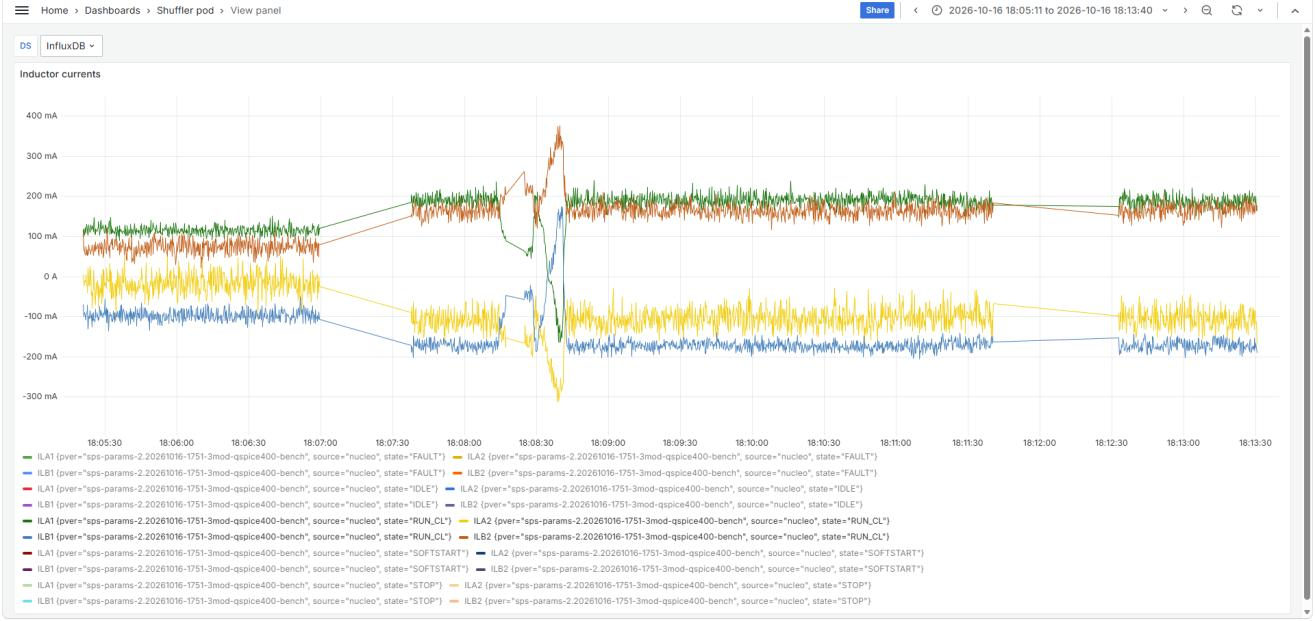
\includegraphics[width=\linewidth]{img-051-119}\caption{Topology and sign conventions.}\end{subfigure}\hfill
  \begin{subfigure}[t]{0.52\linewidth}\centering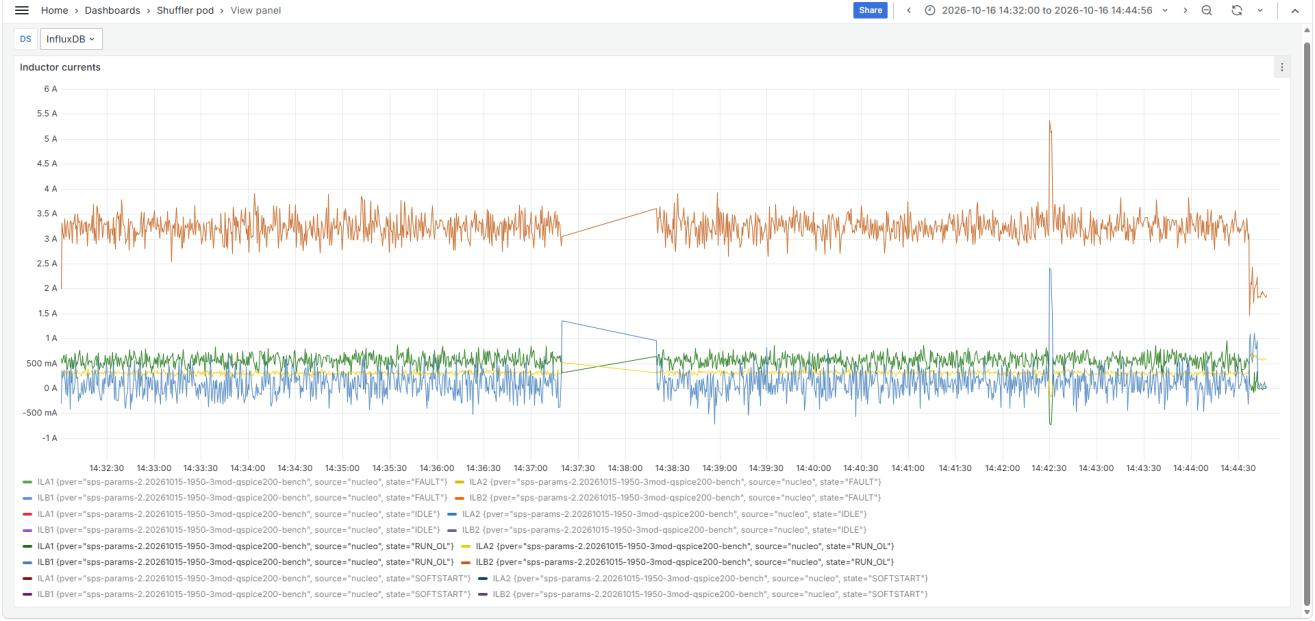
\includegraphics[width=\linewidth]{img-052-123}\caption[{Coupled inductor model}]{Coupled inductor model: $L_k = 0.5L_3$, $L_m = L_2 - 0.5L_3$; ERUC23-4R1K: $R_{DC}$ 1.85\,m$\Omega$, $L_k$ 2.05\,$\mu$H, $L_m$ 5.85\,$\mu$H \cite{tdk_eruc23_ds}.}\end{subfigure}
  \caption{Single-shuffler model elements.}
  \label{fig:single}
\end{figure}

\textbf{State, inputs.} $x = [I_{L1}, I_{L2}, V_{C1}, V_{C2}]^T$, $u_d = [d_A, d_B]^T$, $u_e = [I_{PV1}, I_{PV2}, I_{LOAD}]^T$. $I_{Lk}>0$ flows $V_{mid}\rightarrow L_k\rightarrow$ switch node; $V_{C1} = V_{top}-V_{mid}$, $V_{C2} = V_{mid}$.

\textbf{Switching states.} $2^4=16$ combinations, 7 forbidden (shoot-through), 9 valid; the 4 dual-switch states form the averaged basis with dwell fractions $d_Ad_B$, $d_A(1-d_B)$, $(1-d_A)d_B$, $(1-d_A)(1-d_B)$; the single-switch and all-off states are dead-time transients.

\textbf{Averaged model} (with $\mathbf L = \begin{bmatrix}L & M\\ M & L\end{bmatrix}$):
\begin{align}
  \mathbf L\,\dot{\mathbf I} &= \begin{bmatrix}-d_A V_{C1} + (1-d_A)V_{C2}\\ -d_B V_{C1} + (1-d_B)V_{C2}\end{bmatrix} - R\,\mathbf I\\
  C_1\dot V_{C1} &= d_A I_{L1} + d_B I_{L2} + I_{PV1} - I_{LOAD}\\
  C_2\dot V_{C2} &= I_{PV2} - (1-d_A)I_{L1} - (1-d_B)I_{L2}
\end{align}
Rule: $C_1$ receives current from each phase whose high-side switch conducts; $C_2$ supplies current to each phase whose low-side switch conducts.

\textbf{Equilibrium.} Volt-second balance forces $D_A = D_B \equiv D$ and
\begin{equation}
  \frac{\bar V_{C2}}{\bar V_{C1}} = \frac{D}{1-D},\qquad D = \frac{I_{LOAD}-I_{PV1}}{I_{LOAD}-I_{PV1}+I_{PV2}},\qquad \bar I = \frac{I_{PV2}}{2(1-D)}.
\end{equation}
The differential duty $d_A - d_B$ is a transient input only; a finite load is required for a non-trivial equilibrium.

\textbf{Linearisation and modes.} $\tilde A$ has identical rows 1,2 and columns 1,2 ($L_1 = L_2$). Common-mode duty $\tilde u_c = (\tilde d_A+\tilde d_B)/2$ drives $(I_\Sigma = I_{L1}+I_{L2}, V_{C1}, V_{C2})$; differential duty $\tilde u_\delta = \tilde d_A - \tilde d_B$ drives $I_\Delta = I_{L1}-I_{L2}$ through a pure integrator $L\,\dot{\tilde I}_\Delta = -V_\Sigma \tilde u_\delta$.

\textbf{Stability.} $\sigma(\tilde A) = \{0, 0, \pm j\omega_0\}$, $\omega_0^2 = 2D^2/(LC_1) + 2(1-D)^2/(LC_2)$; with $L = 8.2\uH$, $C = 100\uF$, $D=0.5$: $\omega_0 \approx 34.9$\,krad/s (5.56\kHz), $Z_0 = 0.286\ohm$. With the coupled inductor and $R_w = 1.85$\,m$\Omega$: $-67.3 \pm j26\,968$, $-902$, $0$ ($f_0$ 4.29\,kHz, $\zeta = 0.0025$). The open-loop plant is marginally stable; the controller must provide all damping.

\textbf{Controllability / observability.} Controllable if $\bar I \ne 0$ (no DCM), $V_\Sigma \ne 0$ and $D \in (0,1)$. Observability: $\{V_{C1},V_{C2}\}$ gives rank 3 of 4 (differential current hidden); adding $I_{L1}$ gives rank 4. Per-phase current sensing is therefore mandatory (sensor set of \cref{sec:components}).

\textbf{Discretisation.} ZOH at $T_s = 5\us$: poles $0.9848 \pm 0.1737j$, $1$, $1$ on the unit circle.

\textbf{Cascaded PI (Semester 1 design, superseded).} Crossovers 10\,kHz / 1\,kHz / 5\,kHz, PM 84$^\circ$: $K_{p,i} = 0.00678$, $K_{i,i} = 42.6$; $K_{p,v} = 0.628$, $K_{i,v} = 395$; $K_{p,\delta} = 0.00339$. Three SISO loops treated the coupled states as independent; the fixed-current-reference inner loop drove the shaded module to open circuit (progress report Fig.~8). \Cref{fig:single_portraits} shows the pole map and phase portraits that motivated the MIMO reformulation.

\begin{figure}[htbp]
  \centering
  \begin{subfigure}[t]{0.49\linewidth}\centering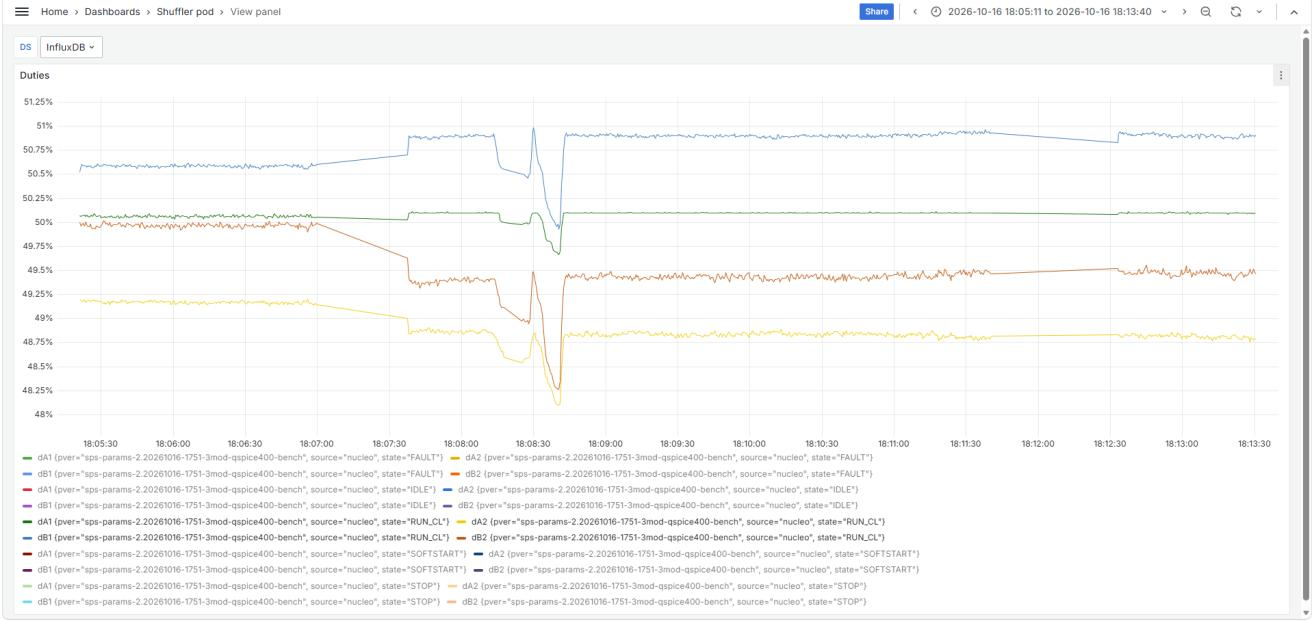
\includegraphics[width=\linewidth]{img-051-121}\caption[{Open-loop eigenvalues}]{Open-loop eigenvalues: idealised model on the $j\omega$ axis; winding resistance and coupling pull the resonant pair into the LHP.}\end{subfigure}\hfill
  \begin{subfigure}[t]{0.49\linewidth}\centering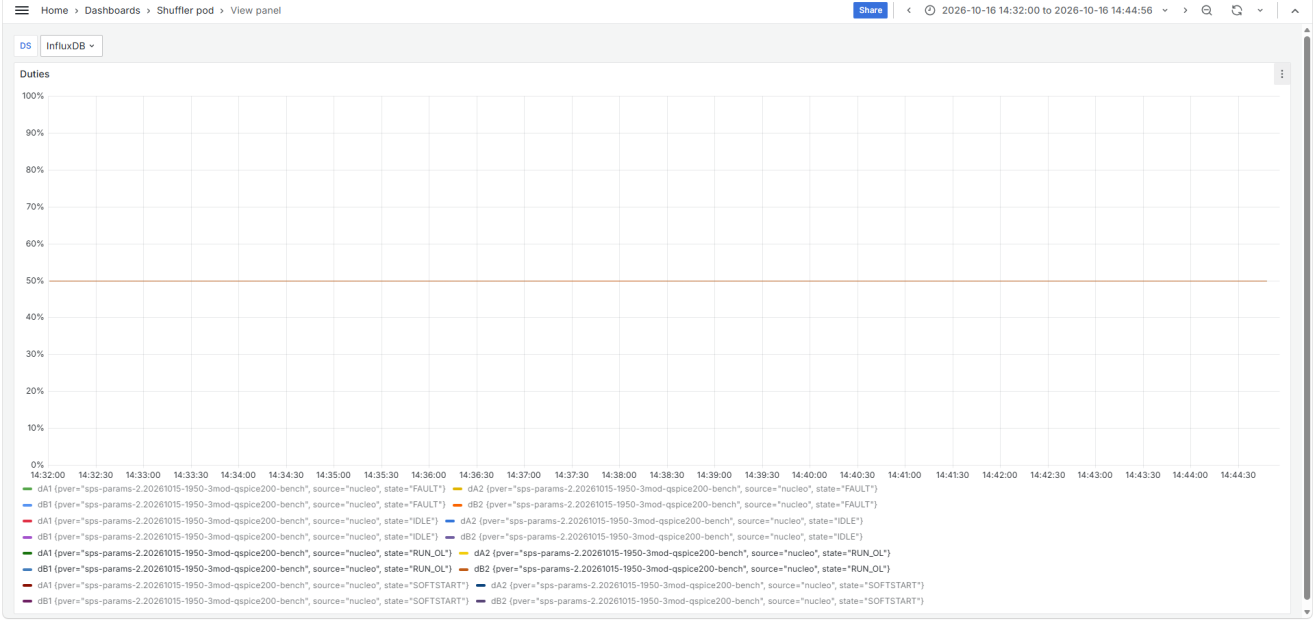
\includegraphics[width=\linewidth]{img-052-125}\caption[{Full 4-state MIMO plant}]{Full 4-state MIMO plant: LQR + integral pulls the resonant pair off the $j\omega$ axis into a well-damped region.}\end{subfigure}\\[3pt]
  \begin{subfigure}[t]{0.75\linewidth}\centering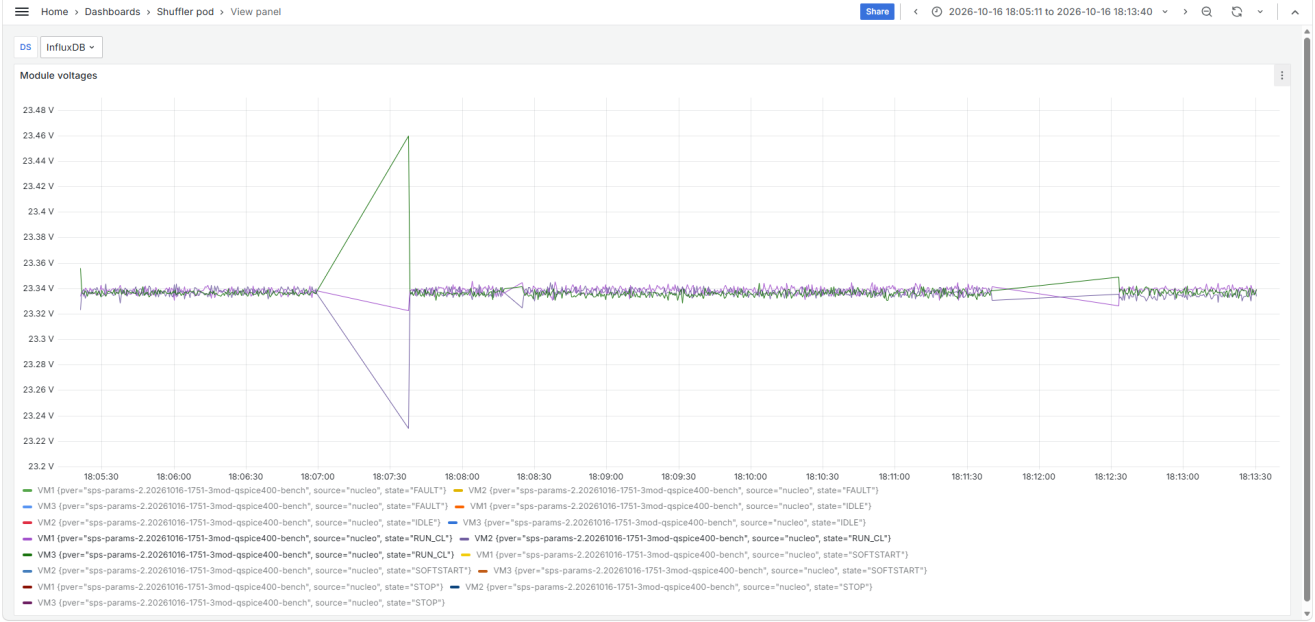
\includegraphics[width=\linewidth]{img-051-120}\caption[{Phase portraits}]{Phase portraits: (a) ideal, centre; (b) passive damping, $\zeta\approx0.003$; (c) inner current loop active, stable focus.}\end{subfigure}
  \caption{Single-shuffler stability pictures (Semester 1 and break).}
  \label{fig:single_portraits}
\end{figure}

\textbf{Re-interpretation after the hardware convention was fixed.} The sensed $I_{LA}+I_{LB}$ \emph{is} the circulating current; relabelled, the Appendix-B model gives $-77$\,V per unit against $-76.5$ measured and $-200$\,A per unit with the 0.386\,$\Omega$ battery-path resistance, so the Semester 1 derivation was right in kind (DESIGN\_LOG 6.1).

\subsection{$N$-module string model (deployed)}
\label{app:nstring}
\begin{figure}[htbp]
  \centering
  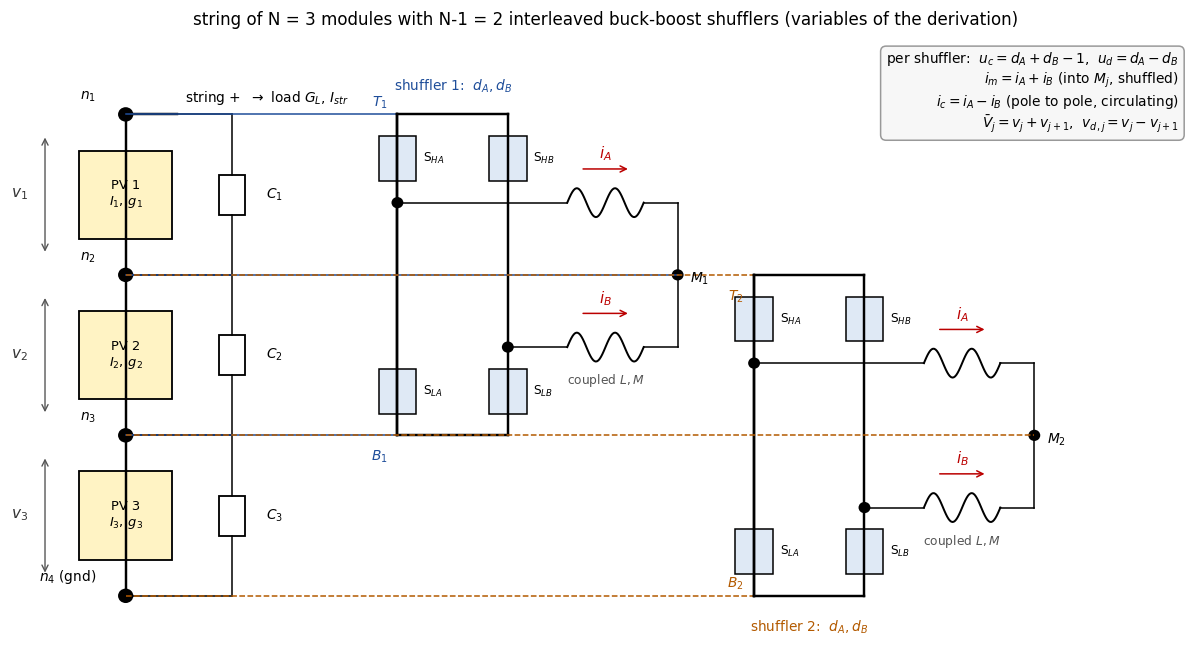
\includegraphics[width=\linewidth]{img-007-011}
  \caption[{Derivation drawing of the $N=3$ string}]{Derivation drawing: $N=3$ modules and $N-1=2$ interleaved buck-boost shufflers with the node potentials and per-shuffler variables of the $N$-module model (the small-signal version is \cref{fig:nodal}).}
  \label{fig:nstring}
\end{figure}
\textbf{Variables} (\cref{fig:nstring}). Node potentials $\phi_k$, $k = 1..N+1$ (node $N+1$ is ground); module voltage $v_k = \phi_k - \phi_{k+1}$. Shuffler $j$ spans modules $j$, $j+1$: rails $\phi_j$, $\phi_{j+2}$, midpoint $\phi_{j+1}$, $\Vbar_j = v_j + v_{j+1}$. Modal duties $\uc = d_A + d_B - 1$, $\ud = d_A - d_B$ (inverse $d_A = \tfrac12(1+\uc+\ud)$, $d_B = \tfrac12(1+\uc-\ud)$). Modal currents $\im = i_A + i_B$ (shuffled; telemetry $I_{LA} - I_{LB}$ because the B sensor is reversed) and $\ic = i_A - i_B$ (circulating; telemetry $I_{LA}+I_{LB}$). Outputs $\vd{}_{,j} = v_j - v_{j+1} = \phi_j - 2\phi_{j+1} + \phi_{j+2}$ and $\ic{}_{,j}$.

\textbf{State equations} (\cref{eq:wind1,eq:wind2,eq:nodal}): $S$ injects $+1$ at the midpoint and $-\tfrac12$ at each rail of shuffler $j$; $G_n$ is the nodal conductance of the module slopes $g_k$ with $G_{load}$ added at node 1; $w$ the module short-circuit current injections. Rail currents are $\tfrac12\im(1\pm\uc) \pm \tfrac12\ic\ud$.

\textbf{Inductances.} As built (ERUC23 windings 1:$-$1) the circulating mode sees $L+M = 13.75\uH$ and the shuffled mode $L-M = 2.05\uH$ ($L_{self} = 7.9\uH$, $M = 5.85\uH$). The ripple law $\Delta\ic = \Vbar/(2\fsw(L+M))$ confirms the assignment (\cref{tab:T6}).

\textbf{Equilibrium.} $D_j\Vbar_j = v_{j+1} + \tfrac12 R_m I_{m,j}$ $\Rightarrow$ $D_j/(1-D_j) = v_{j+1}/v_j$. Charge balance on the ladder: $T(N)\,I_m = \delta I$, $T = \mathrm{tridiag}(-\tfrac12, 1, -\tfrac12)$, $(\delta I)_j = I_j - I_{j+1}$, with the closed form $T^{-1}_{jk} = \tfrac{2}{N}\min(j,k)(N-\max(j,k))$; string current $I_{str} = I_1 - D_1 I_{m,1} = \tfrac1N\sum_k I_k$. For $N=3$: $i_{m1} = (4I_1 - 2I_2 - 2I_3)/3$. Open loop at $D = 0.5$: $\vd{}_{,j} = -R_m \im{}_{,j}$. Check against QSPICE S10i ($R_m = 0.29\ohm$): $\im = -0.466/-0.534\A$ (model) vs $-0.464/-0.539\A$ (QSPICE); $I_{str}$ 1.032 vs 1.024\,A; $R_m\im = -0.135\V$ vs $\vd{}_{,1} = -0.135\V$.

\textbf{DC gain.}
\begin{equation}
  G(N) = \begin{bmatrix} G_v & 0\\ 0 & \mathrm{diag}(\Vbar_j/R_c)\end{bmatrix},\qquad
  G_v = -(R_m I + Z_e)^{-1} Z_e\,\mathrm{diag}(\Vbar_j),\qquad Z_e = -D_v G_n^{-1} S,
\end{equation}
where $D_v$ maps $\phi \mapsto \vd$. $G(2)$: $-\Vbar/(R_m g + 1)$. $G(3)$ voltage block: diagonal $-\Vbar(4R_m g + 3)/(4R_m^2g^2 + 8R_m g + 3)$, off-diagonal $2R_m\Vbar{} g/(\cdot)$: diagonal $\approx -\Vbar$ with $O(R_m g)$ neighbour terms. Numbers in \cref{tab:G}.

\textbf{Controller.} $M = G^{-1}\mathrm{diag}(k_I)$ with $k_{I,v} = 2\pi\cdot150$\,s$^{-1}$, $k_{I,i} = 2\pi\cdot400$\,s$^{-1}$; $u = k\,(M_p e + M\xi)$, $M_p = M\,\mathrm{diag}(k_{p,v},k_{p,v},k_{p,i},k_{p,i})$, $k_{p,v} = 1.58\times10^{-4}$\,s, $k_{p,i} = 1.08\times10^{-4}$\,s, $\xi \mathrel{+}= T_s e$, $T_s = 100\us$, first-order LPF on $y$ with $f_c = 2\kHz$ ($a = 2\pi f_c T_s/(1+2\pi f_c T_s) = 0.557$), one tick of delay; back-calculation anti-windup $\xi = M^{-1}(u_{act} - M_p e)$. Firmware layout $u = [\uc{}_{,1},\uc{}_{,2},\ud{}_{,1},\ud{}_{,2}]$, $e = [e_{vd1}, e_{vd2}, e_{ic1}, e_{ic2}]$. Design: $\tau_v = 1/(k\,k_{I,v})$, $\tau_i = 1/(k\,k_{I,i})$, rise $= 2.197\tau$, 2\,\% settle $= 3.91\tau$.

\begin{table}[htbp]\centering\small
\caption{Design time constants vs gain scale and the closed-loop pole frequencies at $k=1$.}
\label{tab:design_tau}
\begin{tabular}{l r r r l}
\toprule
$k$ & $\tau_v$ [ms] & $\tau_i$ [ms] & rise $2.197\tau_v$ [ms] & closed-loop poles at $k=1$\\
\midrule
0.1 & 10.61 & 3.98 & 23.3 & model $M$: 160 / 164\,Hz ($\vd$), 593\,Hz ($\ic$)\\
0.3 & 3.54 & 1.33 & 7.8 & deployed $M$: 127 / 135\,Hz ($\vd$), 582 / 604\,Hz ($\ic$)\\
1.0 & 1.06 & 0.40 & 2.3 & \\
\bottomrule
\end{tabular}
\end{table}

\textbf{Plants used in the analysis.} PV80 ($N=3$): $V = 20.5\V$, $g = 0.19$\,S per module, $C = [130, 260, 130]\uF$, $G_{load} = 20$\,S (DL3021 CV), $R_w = 0.061\ohm$ (averaged) or $R_{sw}$. BENCH-QSPICE: $V = 23.3\V$, $g = 0$, $I = [0.8, 1.0, 1.3]\A$ (all NGE103 channels in current limit, the 16 Oct point), same $C$. Reduced voltage mode: $f_0 = 1/(2\pi\sqrt{L_m C_e})$ with $C_e = 173\uF$ gives 8.4\,kHz; $\zeta = \tfrac12(R_m\sqrt{C_e/L_m} + g_e\sqrt{L_m/C_e})$ = 0.29 at 61\,m$\Omega$, 1.34 at 0.29\,$\Omega$, 7.8 at 1.7\,$\Omega$.

\textbf{PBH ranks (PV80).} $n = 7$ states; controllable from $u$ (7), from $\uc$ alone (5), from $\ud$ alone (2); observable from $y$ (7), from $\vd$ alone (5): circulating modes are reachable only from $\ud$ and seen only by the current sensors; the string-sum mode (176\,Hz with a current sink) is unreachable/unobservable with equal capacitors and belongs to the load / MPPT. cond$(G(N))$ for PV80 grows only from 16.6 ($N=2$) to 18.9 ($N=8$), i.e.\ the decoupling scales.

\begin{figure}[htbp]
  \centering
  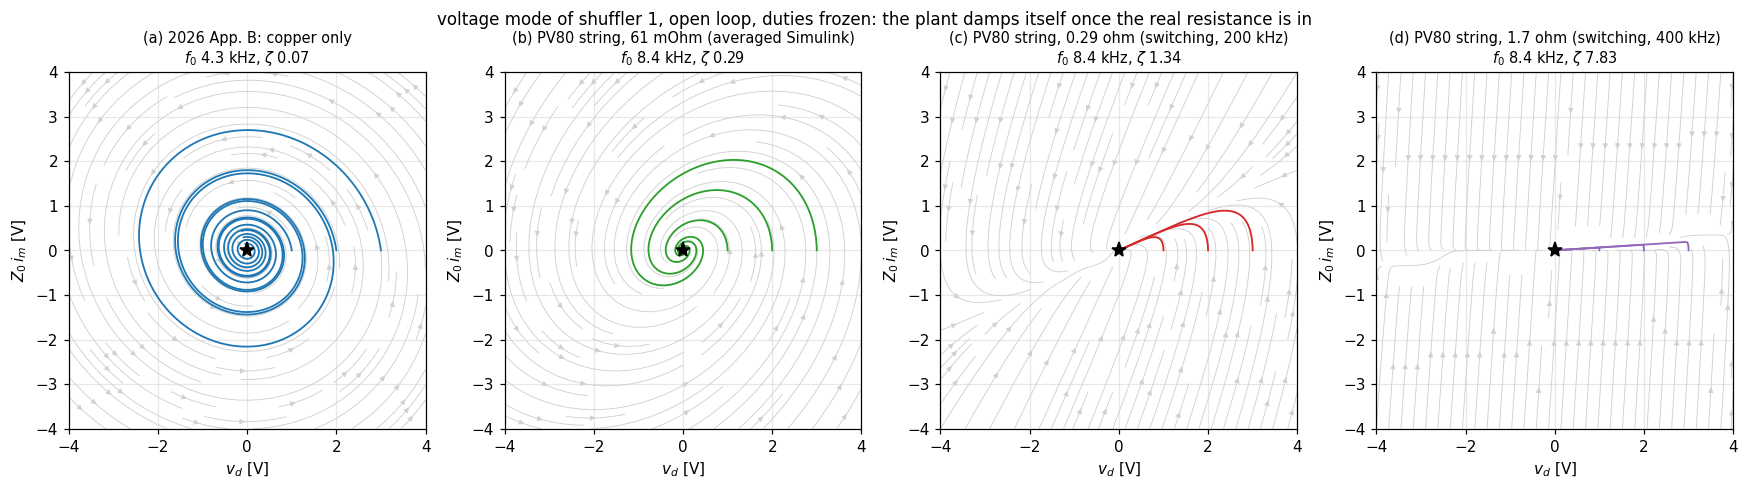
\includegraphics[width=\linewidth]{img-011-012}
  \caption[{Open-loop phase portraits of the voltage mode in the $(\vd,\,Z_0\im)$ plane}]{Open-loop phase portraits of the voltage mode in the $(\vd,\,Z_0\im)$ plane: (a) 2026 App.~B copper-only model ($\zeta\approx0.07$), (b) PV80 plant with the 61\,m$\Omega$ averaged resistance (focus, $\zeta\approx0.3$, 7--9\,kHz), (c) 0.29\,$\Omega$ switching plant at 200\,kHz and (d) 1.7\,$\Omega$ at 400\,kHz (over-damped nodes). The plant damps itself once the real switching resistance is included.}
  \label{fig:ana_portraits}
\end{figure}

\begin{figure}[htbp]
  \centering
  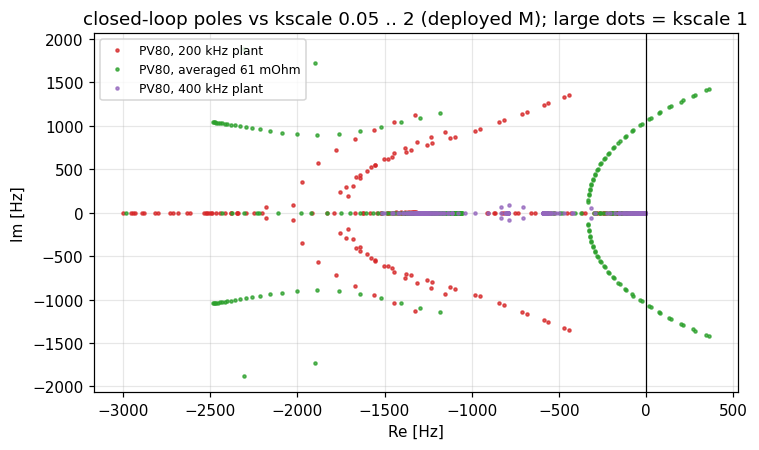
\includegraphics[width=0.68\linewidth]{img-012-014}
  \caption[{Closed-loop poles of the analytical $N=3$ model as the gain scale $k$ is swept}]{Closed-loop poles of the analytical $N=3$ model with the deployed gain set as $k$ is swept from 0.05 to 2, for the 200\,kHz (0.29\,$\Omega$), averaged (61\,m$\Omega$) and 400\,kHz (1.7\,$\Omega$) plants; large dots mark $k=1$.}
  \label{fig:ana_rl}
\end{figure}

\subsection{Switching resistance $R_{sw}$}
\label{app:rsw}
The averaged 61\,m$\Omega$ plant over-predicts the current-loop gain $5\times$. Open-loop $\ud$ sweeps on the QSPICE device model (S10i / S10i3 / S10i4) with and without reverse recovery and device capacitances isolate the mechanism: pole-capacitance commutation during the dead time costs volt-seconds proportional to the current,
\begin{equation}
  R_{sw} = \frac{4\Vbar^2 C_p \fsw}{\Delta i^2} = 64\,C_p\,\fsw^3\,(L+M)^2,
\end{equation}
which with $C_p = 2.2$\,nF gives 0.21 / 0.72 / 1.70\,$\Omega$ at 200 / 300 / 400\,kHz; the identified gains (142 / 58 / 23\,A per unit) imply 0.27 / 0.79 / 1.66\,$\Omega$; the analysis uses 0.29 / 0.80 / 1.70\,$\Omega$. The switching twin (\code{nswitch.py}, exact per-configuration integration with $C_p = 2C_{oss}$) reproduces QSPICE point for point (170/165/148/111/74/66 vs 172/163/148/112/71/66\,A per unit).

\subsection{Open items}
Unexplained 6.34\,kHz / $\zeta$ 0.53 resonance seen in June 2026; $C_{oss}$ is voltage dependent so $R_{sw}$ should be re-measured per operating point; the $\ud\rightarrow\vd$ cross term ($-10\ldots-25$\,V per unit) is not in the model; at 400\,kHz the dead time sits at the ZVS boundary and the linear model stops near $\ud\approx0.02$.
